\documentclass[answers, 10pt]{exam}
\usepackage[french]{babel} 
\usepackage[]{amsmath,amssymb}
\usepackage[]{cleveref} 
\usepackage[]{cancel} 
\usepackage[]{minted}
\usepackage{graphicx}
\usepackage[]{subcaption}
\usepackage{caption}
\graphicspath{{./src/}}

\begin{document}

\title{RO05 - \'Evolution de la valeur d'un actif financier}
\author{Maxime Delboulle, Pascal Quach}
\maketitle

Considérons une option européenne représentant un actif financier dont la
valeur au temps $t$ est $S(t)$ pour $0 \leq t \leq T$, où $T$ est le temps de
l’exercice de l’option. 

Notons $M\in \mathbb{N}^*$ le nombre de sous-divisions de l’intervalle $[0, T]$
et $h=\frac{T}{M}$.  

Notons également $S_n = S(nh)$, pour $n=0, \dots, M$, les valeurs de l’actif
aux instants $t= nh$.  L’équation d’évolution du prix de l’actif en temps
discret s’écrit comme suit :

\begin{equation}\label{eq:actif-financier}
	S_{n+1} = S_n + \mu h S_n + \sigma h^{ \frac{1}{2} } S_n \xi_n,\quad n \geq 0 
\end{equation}

où $\xi_n, n\geq 0$ est une suite de v.a. iid de loi $\mathcal{N}(0, 1)$
indépendante de $S_0$.

\begin{questions}
	\question 
	Expliquer la construction de \cref{eq:actif-financier}.

	\begin{solutionorbox}
		Ici, on note la modélisation suivante~:
		
		\begin{itemize}
			\item $S(t)$, la valeur de l'actif financier au temps $t$.
			\item $\mu$, le taux d'intérêt de l'actif
			\item $\sigma$, la volatilité de l'actif
			\item $(\xi_n)_{n\geq 0}$ représente du bruit
		\end{itemize}

		Dans l'équation d'évolution, chaque terme représente
		respectivement le capital à l'instant présent, l'évolution de
		l'actif et la volatilité stochastique~:

		\begin{equation*}
			S_{n+1} = \underbrace{S_n}_{\text{valeur précédente}} 
			+ \underbrace{\mu h S_n}_{\text{intérêt}} 
			+ \underbrace{\sigma h^{ \frac{1}{2} } S_n \xi_n}_{\text{bruit}}
			,\quad n \geq 0 
		\end{equation*}

	\end{solutionorbox}

	\question
	Montrer que

	\begin{equation*}
		S_M = S_0 \prod_{n=0}^{M-1} (1 + \mu h + \sigma h^{\frac{1}{2}} \xi_n
)		,
	\end{equation*}

	et en déduire que 

	\begin{equation*}
		\ln \left( \frac{S_M}{S_0} \right) = \sum_{n=0}^{M-1} \ln(1 + \mu h + \sigma h^{\frac{1}{2}} \xi_n).
	\end{equation*}

	\begin{solutionorbox}
		Pour $M\in \mathbb{N}^*$ fixe, on factorise $S_M$ tel que 
		\begin{equation*}
			S_M = \left[ 1 + \mu h + \sigma h^{\frac{1}{2}} \xi_{n}\right] S_{M-1}
		\end{equation*}	

		Par récurrence,

		\begin{equation*}
			S_M = S_0 \prod_{n=0}^{M-1}  (1 + \mu h + \sigma h^{\frac{1}{2}}\xi_n
) 		\end{equation*}
		
		Alors, on obtient,
		\begin{equation}\label{eq:q2}
			\ln \left( \frac{S_M}{S_0} \right) = \sum_{n=0}^{M-1} \ln(1 + \mu h + \sigma h^{\frac{1}{2}} \xi_n)
			,
		\end{equation}

		car on fait l'hypothèse que $\forall n \geq 0 : S_M > S_0 > 0$. De même, pour calculer la somme des log, on doit avoir
		
		$$\forall n \geq 0 : 1 + \mu h + \sigma h^{\frac{1}{2}} \xi_n > 0 \iff \forall n \geq 0 : \xi_n > \frac{-1 + \mu h^{\frac{1}{2}}}{\sigma}  $$
		Ces inégalités ne sont pas systématiquement vérifiées pour tout n. On en fait l'hypothèse.

	\end{solutionorbox}

	\question

	En utilisant l'approximation $\ln(1 + \varepsilon) \approx \varepsilon - \frac{\varepsilon^2}{2}$, pour $\varepsilon \to 0$, et la loi des grands nombres, montrer que

	\begin{equation*}
		\ln \left(  \frac{S(t)}{S_0} \right) \approx \left( \mu - \frac{1}{2} \sigma^2 \right)t.
	\end{equation*}

	Ici, on a supposé que l'approximation proposée est valable lorsque $h\to 0$.

	\begin{solutionorbox}
		On note $\varepsilon = \mu h + \sigma h ^{\frac{1}{2}} \xi_k$,
		pour un $k\in \mathbb{N}^*$ fixé.

		Alors,

		\begin{align}\label{eq:approx}
			\ln \left( 1 + \mu h + \sigma h^{\frac{1}{2}}\xi_k \right) &\approx \mu h + \sigma h^{\frac{1}{2}} \xi_k - \frac{1}{2} \left( \mu h + \sigma h^{\frac{1}{2}}\xi_k \right)^2\\
										   &\approx \mu h + \sigma h^{\frac{1}{2}} \xi_k - \frac{1}{2} \left( \cancel{\mu^2 h^2} + \cancel{2\mu h^{\frac{3}{2}}} \xi_k  + \sigma^2 h \xi_k^2 \right) & h\to 0, h\ggg h^{1 + \delta}, \delta > 0
\\
									      &\approx \mu h + \sigma h^{\frac{1}{2}} \xi_k - \frac{1}{2} \sigma^2 h \xi_k^2 	
		\end{align}

		Le résultat précédent (\cref{eq:q2}) est valable pour tout
		$n=0,\dots,M$.

		Finalement, en remplaçant l'approximation obtenue dans
		\cref{eq:q2}, on obtient~:

		\begin{align*}
			\ln \left(  \frac{S(t)}{S_0} \right) &\approx \sum_{n=0}^{M-1}\left(  h\mu + \sigma h^{\frac{1}{2}} \xi_n - \frac{1}{2} \sigma^2 h \xi_n^2 \right)  \\
							     &\approx M h\mu + \sigma h^\frac{1}{2} \sum_{n=0}^{M-1} \xi_n - \frac{1}{2} \sigma^2 h \sum_{n=0}^{M-1} \xi_n^2 & \text{LGN}\\
							     &\approx M h \mu + \sigma M h^\frac{1}{2} \underbrace{\mathbb{E}\left[ \xi_n \right]}_{0} - \frac{1}{2} \sigma^2 Mh\underbrace{\mathbb{E}\left[ \xi_n^2 \right]}_{\text{Var}\left[\xi_n \right] - (\mathbb{E}\left[\xi_n \right])^2 } & (\xi_n)_{n\geq 0} \sim \mathcal{N}(0, 1)\\
							     &\approx \left(\mu - \frac{1}{2} \sigma^2  \right) \underbrace{Mh}_{t}\\
				\ln \left(  \frac{S(t)}{S_0} \right) &\approx \left(\mu - \frac{1}{2} \sigma^2  \right) t & \blacksquare\\
		\end{align*}
	\end{solutionorbox}

	\question
	\`A l'aide du théorème de la limite centrale, montrer que l'approximation ci-dessus peut se préciser plus par la relation

		\begin{equation*}
			\ln \left( \frac{S(t)}{S_0} \right) \sim \mathcal{N} \left(  \left(  \mu - 1/2 \sigma^2 \right)t, \sigma^2 t \right).
		\end{equation*}
	
	\begin{solutionorbox}
		En notant la suite de v.a. iid $(X_n)_{n=0,\dots,M}$, avec $X_n = \ln \left( 1 + \mu h + \sigma h^\frac{1}{2} \xi_n \right)$, on applique le théorème centrale limite~:
		\begin{align*}
			X_{1} + \dots + X_{M} \sim \mathcal{N}\left(M \mathbb{E}\left[X_1 \right], M \text{Var}\left[X_1 \right]\right)
		\end{align*}

		à 

		\begin{equation*}
			\ln \left(  \frac{S(t)}{S_0} \right) \approx \sum_{n=0}^{M-1}\left(  h\mu + \sigma h^{\frac{1}{2}} \xi_n - \frac{1}{2} \sigma^2 h \xi_n^2 \right)
		\end{equation*}

		Alors, 

		\begin{align*}			
			\mathbb{E}\left[\mu h + \sigma h^{\frac{1}{2}} \xi_n - \frac{1}{2} \sigma^2 h \xi_n^2\right] &= \mu h + \sigma h^{\frac{1}{2}} \underbrace{\mathbb{E}\left[\xi_n \right]}_{0} - \frac{1}{2} \sigma^2 h \underbrace{\mathbb{E}\left[ \xi_n\right]}_{1}\\
													  \mathbb{E}\left[X_1 \right] &= h \left( \mu - \frac{\sigma^2}{2} \right)\\
													  M\mathbb{E}\left[X_1 \right] &= \underbrace{Mh}_{t} \left( \mu - \frac{\sigma^2}{2} \right)
		\end{align*}

		\begin{align*}
			\text{Var}\left[X_1 \right] &= \mathbb{E}\left[X_1^2 \right] - \left( \mathbb{E}\left[X_1 \right] \right)^2\\
						    &= \mathbb{E}\left[\left(\mu h + \sigma h^{\frac{1}{2}} \xi_n - \frac{1}{2} \sigma^2 h \xi_n^2 \right)^2 \right] - h^2 \left( mu - \frac{\sigma^2}{2} \right)^2 & h\to 0, h\ggg h^{1 + \delta}, \delta > 0\\
						    &= \mathbb{E}\left[\sigma^2 h \xi_n \right]\\
			\text{Var}\left[X_1 \right] &= h\sigma^2\\
			M \text{Var}\left[X_1 \right] &= \underbrace{Mh}_{t}\sigma^2\\
		\end{align*}	

		Finalement,

		\begin{equation*}
			\ln \left( \frac{S(t)}{S_0} \right)\sim \mathcal{N} \left( \left( \mu - \frac{\sigma^2}{2}\right)t, \sigma^2 t\right)
		\end{equation*}

	\end{solutionorbox}

	\question
	Conclure de la question précédente que
	\begin{equation*}
		S(t) = S_0 \exp \left(  \left(  \mu - \frac{1}{2}\sigma^2 \right)t + \sigma \sqrt{
		t}Z \right),
	\end{equation*}

	où $Z\sim \mathcal{N}(0, 1)$.
	
	\begin{solutionorbox}
		On pose :
		\begin{itemize}
			\item $Y=\ln \left( \frac{S(t)}{S_0} \right)$,
			\item $\mu' = \left( \mu - \frac{1}{2} \sigma^2 \right)t$,
			\item $\sigma' = \sigma \sqrt{t}$,
			\item $Z = \frac{Y - \mu'}{\sigma'} \sim \mathcal{N}(0, 1)$
		\end{itemize}

		ce qui donne immédiatement 

		\begin{align}%
			\label{eq:st}
			S(t) = S_0\exp \left( \left( \mu - \frac{1}{2}\sigma^2 \right)t + \sigma \sqrt{t}Z\right)
		\end{align}
		
	\end{solutionorbox}

	\question
	Expliquer pourquoi la v.a. $\frac{S(t)}{S_0}$, ($T$ fixé) suit-elle une
	loi log-normale ? Spécifier ses paramètres.
	
	\begin{solutionorbox}
		Si $X\sim \mathcal{N}(\mu, \sigma^2)$, alors, $\exp(X)\sim
		\text{LN}(\mu, \sigma^2)$.

		Ici, en considérant $Y =\ln \left( \frac{S(t)}{S_0} \right) = 
		\frac{Z - \mu'}{\sigma'}\sim \mathcal{N}(\mu', \sigma'^2)$, 
		on obtient alors,

		\[
			\frac{S(t)}{S_0}\sim \text{LN}\left( 
			\left( \mu - \frac{1}{2}\sigma^2 \right)t, \sigma^2 t
			\right)
		.\] 


	\end{solutionorbox}

	\question
	Donner un intervalle de confiance de valeur l'option au temps
	d'exercice au niveau $\alpha$.

	\begin{solutionorbox}
		On calcule un intervalle de confiance bilatéral pour $Z$, et on
		en déduit l'intervalle de confiance pour $S(t)$.

		On note $u_{\alpha} = \Phi^{-1}(\alpha)$, le quantile d'ordre
		$\alpha$ de la loi normale centrée-réduite.

		Alors,
		\[
			Z = \frac{1}{\sigma'} \left( 
				\ln\left( \frac{S(t)}{S_0}\right) - \mu' 
			\right)
		.\] 

		\begin{align*}
			\mathbb{P}\left( u_{\alpha / 2} \leq Z \ \leq u_{1 - \alpha / 2} \right) &= 1 - \alpha & u_\alpha \text{ symétrique}\\
			\mathbb{P}\left( u_{\alpha / 2} \leq \frac{1}{\sigma'}\left( \ln\left( \frac{S(t)}{S_0}\right) - \mu' \right) \leq u_{1 - \alpha / 2} \right) &= 1 - \alpha & \sigma' > 0\\
			\mathbb{P}\left( S_0\exp\left(\sigma'u_{\alpha / 2} + \mu'\right) \leq S(t) \leq S_0\exp\left(\sigma'u_{1 - \alpha / 2} + \mu'\right) \right) &= 1 - \alpha & \exp\text{ strictement croissante}\\
		\end{align*}

		Donc l'intervalle de confiance au niveau $\alpha$ pour $S(t)$ est \[
			\text{IC}_\alpha = \left[ S_0\exp\left(\sigma\sqrt{t}u_{\alpha / 2} + \left( \mu - \frac{1}{2} \sigma^2 \right)t\right); S_0\exp\left(\sigma\sqrt{t}u_{1 - \alpha / 2} + \left( \mu - \frac{1}{2} \sigma^2 \right)t\right)\right]
		.\] 
	\end{solutionorbox}

	\question
	
	\textit{Monte Carlo.} Effectuer 1000 réalisations des v.a. $S_n$, pour
	$n=0,\dots,M$, et donner l'évolution moyenne de la valeur de l'actif.
	Les données sont : 
	
	\begin{itemize}
		\item $T=1$
		\item $h = 0.05$
		\item $S_0 = 1$
		\item $\mu = 0.05$
		\item $ \sigma = 0.3$
	\end{itemize}

	\begin{solutionorbox}
	\begin{minted}[breaklines, frame=single]{python}
import numpy as np ; import math ; from scipy.stats import norm

# paramètres du problème
mu = 0.05 ; alpha = 0.1
sigma = 0.3 ; sigma2 = sigma**2
S0 = 1 ; h = 0.05 ; T = 1
M = int(T/h) ; N = 1000

def get_IC (t) :
    """ get IC """    
    return (S0 * np.exp(
                    sigma * math.sqrt(t) * np.array([norm.ppf(alpha/2), norm.ppf(1 - alpha/2)]) + 
                    (mu - sigma2/2) * t))
def get_S_t () :
    """ retourne une liste de S(t) ; t allant de 1 à M. et intervalle de confiance IC """
    Z = np.random.rand(M)
    SM =[
        S0 * np.exp((mu - sigma2/2) * t + sigma * np.sqrt(t) * Z[t])
        for t in range(M)]
    IC = np.array([get_IC(t) for t in range(M)])
    return {"SM":SM, "IC":IC}

# génération d'une liste de N échantillons S(t) ; t allant de 1 à M
SMN = np.array([get_S_t()["SM"] for n in range(N)])

# affichage du gain moyen de l'actif boursier de 1 à M (N éléments)
print(f"gain moyen: {(SMN[:, -1] - S0).mean():.2f}")

\end{minted}
		
Le gain  moyen est de 1,3. Nous obtenons finalement les courbes suivantes :

\includegraphics[width=0.45\linewidth]{échantillon.png}
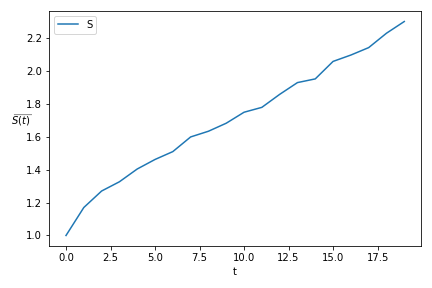
\includegraphics[width=0.45\linewidth]{moyenne.png}
\captionof{figure}{le graphique de gauche représente l'évolution de 4 actifs financiers avec un intervalle de confiance à 90 \%. La figure de droite représente l'évolution moyen de 1.000 actifs.}

\end{solutionorbox}
\end{questions}

\end{document}
